\documentclass[10pt,twocolumn]{article}

% use the oxycomps style file
\usepackage{oxycomps}

% usage: \fixme[comments describing issue]{text to be fixed}
% define \fixme as not doing anything special
\newcommand{\fixme}[2][]{#2}
% overwrite it so it shows up as red
\renewcommand{\fixme}[2][]{\textcolor{red}{#2}}
% overwrite it again so related text shows as footnotes
%\renewcommand{\fixme}[2][]{\textcolor{red}{#2\footnote{#1}}}

% read references.bib for the bibtex data
\bibliography{references}

% include metadata in the generated pdf file
\pdfinfo{
    /Title (The Occidental Computer Science Comprehensive Project: Goals, Timeline, Format, and Advice)
    /Author (Justin Li)
}

% set the title and author information
\title{Tutorial Report - Captcha Reader}
\author{Luis Martinez}
\affiliation{Occidental College}
\email{lmartinez3@oxy.edu}

\begin{document}

\maketitle

\section{Introduction}

For my upcoming comps project, I am planning to develop a handwritten-text identifier that enables users to scan handwritten documents and convert them into searchable PDFs while preserving the original formatting. The primary audience for this is students who prefer handwriting notes, as it gives the convenience of searching for specific topics that are otherwise unavailable to them. If time permits, I also intend to incorporate a feature allowing users to highlight specific text with a yellow highlighter, which would then be automatically added to a table of contents within the PDF. Currently, I plan to leverage machine learning to accomplish this Project. 

For my tutorial, I have chosen "OCR model for reading Captchas" by Aakash Kumar Nain from Keras (\href{https://keras.io/examples/vision/captcha_ocr/}{https://keras.io/examples/vision/captcha\_ocr/}) with additional information from "OCR model for reading Captchas - Keras Code Examples" by Connor Shorten (\href{https://www.youtube.com/watch?v=SHo3hbsJs_U}{https://www.youtube.com/watch?v=SHo3hbsJs\_U}). The goal of this tutorial is to create a model that can take an image of a Captcha and accurately output the text. This tutorial is relevant to my comps project because handwritten text recognition is already well studied and, since I want to take that code a step further, I have to understand how current handwriting recognition is done. The tutorial's goal is to create a program capable of effectively interpreting Captchas using a simple OCR (Optical Character Recognition) model.


\section{Method}
\subsection{Setup}
The first step of the tutorial is to import the necessary libraries and set up the environment for building and training machine learning models. The OS module is required to set up the environment variable for \texttt{KERAS\_BACKEND} to \texttt{tensorflow}. \texttt{numpy}, \texttt{matplotlib}, \texttt{pathlib}, and \texttt{Counter} are all basic imports for data manipulation, visualization and file handeling tasks. Finally, \texttt{tensorflow}, \texttt{keras}, and \texttt{layers} are open-source machine learning libraries which we need to do neural networks for this tutorial

\subsection{Load the Data}
The next step is to load in the data from a Github Repository by defining the path to the directory containing the captcha images. Next, it extracts the labels for each image by parsing the file paths. The labels are derived from the filenames of the images, removing the directory path and file extension. This dataset is contains 1040 Captcha pngs. Notably, this dataset only has 19 unique characters which will limit what the model will be able to identify. This is determined by iterating over each label, extracting individual characters, and adding them to a set to eliminate duplicates.Additionally, this section of code defines the batch size as 16, and it defines the size of the images as being 50 x 200 which also limits the images that it can identify. These parameters are essential for standardizing the input data and configuring the model architecture appropriately.


\subsection{Preprocessing}
For this section, we have to create two dictionaries: \texttt{char\_to\_number} and \texttt{num\_to\_char}, which map characters to integers and integers back to the original characters, respectively. This is crucial for converting text labels into a numerical format suitable for training the model. The \texttt{split\_data} function takes arrays of image paths and corresponding labels as input and splits them into training and validation sets. This step ensures that the model can learn from a portion of the data while being evaluated on another portion to assess its performance. The \texttt{encode\_single\_sample} function reads an image file, decodes it, converts it to grayscale, resizes it to the desired dimensions, and transposes it. Additionally, it maps characters in the label to their corresponding integers using the \texttt{char\_to\_num} dictionary. This function prepares individual samples in a format suitable for feeding into the OCR model during training.



\subsection{Create Dataset Objects}
In this section \texttt{Dataset} objects are created for \texttt{Tensorflow} for the training and validation sets. The code creates a \texttt{Dataset} object for the training dataset using \texttt{tf.data.Dataset.from\_tensor\_slices((x\_train, y\_train))}. This function slices the input arrays \texttt{x\_train} (containing images) and \texttt{y\_train} (containing corresponding labels) along the first dimension to create a dataset of image-label pairs. Next, the \texttt{encode\_single\_sample} function is applied to each sample in the training dataset using the \texttt{map} method. This function performs preprocessing on each sample, such as reading the image file, decoding it, resizing it, and encoding the label characters to integers. After preprocessing, the dataset is batched using the \texttt{batch} method with a specified batch size (\texttt{batch\_size}). Batching groups multiple samples together into batches, which helps in optimizing computation during training by processing multiple samples simultaneously. Finally, the \texttt{prefetch} method is used to prefetch data from the dataset, allowing for parallel data loading and processing. The \texttt{buffer\_size} argument determines the number of elements to prefetch, which helps to keep the data pipeline running smoothly by reducing the time spent waiting for data.


\subsection{Visualize Data}

This is pretty standard code for visualizing images in Google Colab.


\subsection{Model}

The this code contains the functions and a custom Keras layer tailored for computing the Connectionist Temporal Classification (CTC) loss. The \texttt{ctc\_batch\_cost} function computes the CTC loss utilizing true labels (\texttt{y\_true}), predicted probabilities (\texttt{y\_pred}), input sequence lengths (\texttt{input\_length}), and label lengths (\texttt{label\_length}). It involves converting data types and dimensions for label and input lengths which transforms the true labels into a sparse representation through \texttt{ctc\_label\_dense\_to\_sparse}, and computing the CTC loss via TensorFlow's \texttt{tf.nn.ctc\_loss}. The \texttt{ctc\_label\_dense\_to\_sparse} function reshapes and masks dense labels to create the necessary sparse representation mandated by the CTC loss calculation. The \texttt{CTCLayer} class defines a custom Keras layer encapsulating CTC loss computation, initialized with \texttt{ctc\_batch\_cost}, and incorporates the computed loss into the layer's losses to ensure its inclusion in the overall model loss. The \texttt{build\_model} function constructs an OCR model integrating CNNs, RNNs, and the custom \texttt{CTCLayer}, comprising convolutional layers followed by bidirectional LSTM layers and a dense output layer, with the \texttt{CTCLayer} serving as the output layer to compute the CTC loss during training. 



\subsection{Training}

This section is standard model training code with 100 epochs (one complete pass through the entire training dataset).


\subsection{Inference}

The code includes the functions and operations associated with decoding the output of the OCR model and visualizing the results. The \texttt{ctc\_decode} function takes the predicted probabilities (\texttt{y\_pred}), input lengths (\texttt{input\_length}), and optional parameters for decoding strategy (greedy or beam search). Initially, it computes the logarithm of the predicted probabilities, reshaping the input based on the shape of \texttt{y\_pred}, and then executes either greedy decoding via \texttt{tf.nn.ctc\_greedy\_decoder} or beam search decoding using \texttt{tf.compat.v1.nn.ctc\_beam\_search\_decoder}, contingent on the \texttt{greedy} parameter value. The decoded sequences are converted into dense representations and returned along with the log probabilities. Subsequently, the code extracts the prediction model from the main model (\texttt{model}) up to the output layer (\texttt{dense2}) and defines a utility function \texttt{decode\_batch\_predictions}. This function accepts the model predictions (\texttt{pred}) and decodes them using the \texttt{ctc\_decode} function, assuming a greedy decoding strategy. It iterates over the decoded sequences, converts them into text using a character mapping, and appends them to an output list. Finally, the code demonstrates the decoding results on some validation samples by iterating over a batch of validation data, obtaining predictions from the prediction model, decoding them using the \texttt{decode\_batch\_predictions} function, and visualizing the original images alongside their predicted texts using Matplotlib which enables a qualitative assessment of the OCR model's performance on unseen data.
\begin{figure}
    \centering
    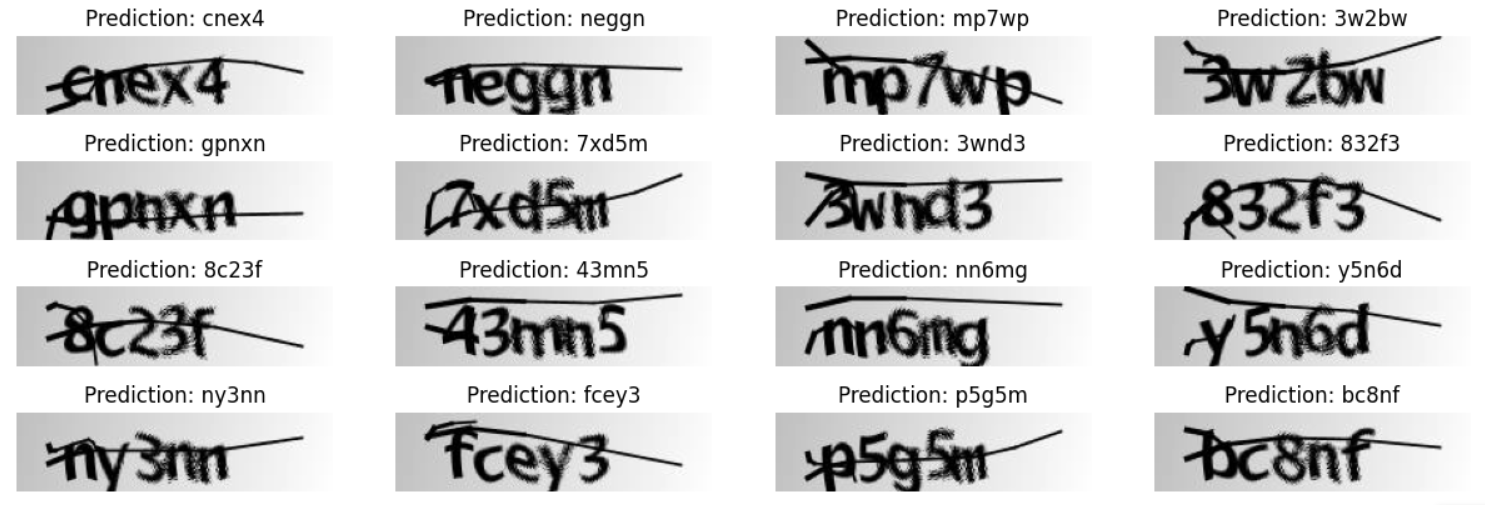
\includegraphics[width=1\linewidth]{captcha results.png}
    \caption{Model Results}
    \label{fig:enter-label}
\end{figure}
\subsection{Accuracy Code}
In addition to the code provided I also added this code to simply calculate the accuracy of the model. It iterates over the validation dataset, makes predictions, compares the predictions with the ground truth labels, and calculates the accuracy. This accuracy calculation is done separately after training the model.

\section{Metrics and Results}
Running the Accuracy Code outputs an 0.9903846153846154, which actually seems too high for a machine learning model. However, the prevalence of text recognition software and the limited number of unique characters makes me comfortable accepting this result. Furthermore, the output from the Inference code segment confirms this accuracy (Figure 1). Thus, I am confident in saying that I accomplished the goal of the tutorial. 


\section{Reflection}
After completing this tutorial, I am very confident in the fact that I need to do significantly more research in the coming months, including but not limited to researching what file format will be best for copying the format of the original scanned document.  Additionally, I'll need to invest time in finding a more comprehensive model that encompasses all English characters or, alternatively, develop a model myself. Considering the limitations highlighted in the tutorial, it's likely that scanning an entire document at once might not be feasible given the specific sizes of most Captcha model datasets.  I anticipate that I'll have to use a model to scan individual sections of the uploaded document and subsequently stitch-together the results. Regarding concerns, I don't have experience modifying file types like pdfs or docxs directly with code, nor do I have experience in actually using a machine learning model within a program. Therefore, I'm mostly worried about whether or not I have enough time and energy to learn and apply this information in the given time-frame. 

\printbibliography

\end{document}
